\chapter{Simple Machines}

As mentioned earlier, physicists define work to be the force applied
times the distance it is applied over. So, if you pushed your car 100
meters with 17 newtons of force, you have done 1700 joules of work.

Humans have always had to move really heavy things, so many centuries
ago we developed simple machines to decrease the amount of force
necessary to execute those tasks. These include things like:
\begin{itemize}
\item Levers
\item Pulleys
\item Ramps
\item Gears
\item Hydraulics
\item Screws
\end{itemize}
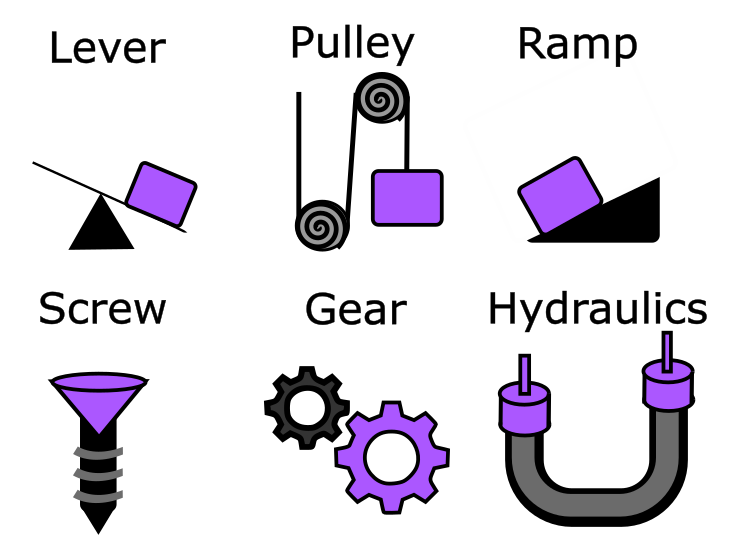
\includegraphics[width=0.8\textwidth]{Simple_Machines.png}

While these machines can decrease the force needed, they don't change
the amount of work that must be done. So if the force is decreased to
a third, the distance that you must apply the force is increased by a
factor of three.

``Mechanical gain'' is what we call the increase in force.

\section{Levers}

A lever rotates on a fulcrum. To decrease the necessary force, the load
is place nearer to the fulcrum than where the force is applied.

In particular, physicsts talk about the \newterm{torque} created by a
force. When you push on a lever, the torque is the product of the
force you exert and the distance from the point of rotation.

Torque is typically measured in newton-meters.

To balance two torques, the products must be the same. So, assuming
that the forces are applied in the proper direction,

$$R_L F_L = R_A F_A$$

where $R_L$ and $R_A$ are the distance from the fulcrum to the where
the load's force and the applied force (respectively) are applied, and
$F_L$ and $F_A$ are the amount of the forces.

\begin{Exercise}[title={Lever}, label=lever]
  
Paul, who weighs 70 kilograms, sits on a see-saw 4 meters from the
fulcrum.  Jan, who weights 50 kilographs, wants to balance. How far
should Jan sit from the fulcrum?

\end{Exercise}
\begin{Answer}[ref=lever]
  Paul is exerting $(70)(9.8)$ newtons of force at 4 meters from the
  fulcrum, so he is creating a torque of 2,744 newton-meters of torque
  on the see-saw.  Jan is creating $(50)(9.5) = 490$ newtons of
  force.

  If $r$ is the distance from the fulcrum to Jan's seat, to balance
  $490 r = 2744$, so $r = 5.6$ meters.
\end{Answer}
% KA: https://www.khanacademy.org/science/physics/discoveries/simple-machines-explorations/a/lever
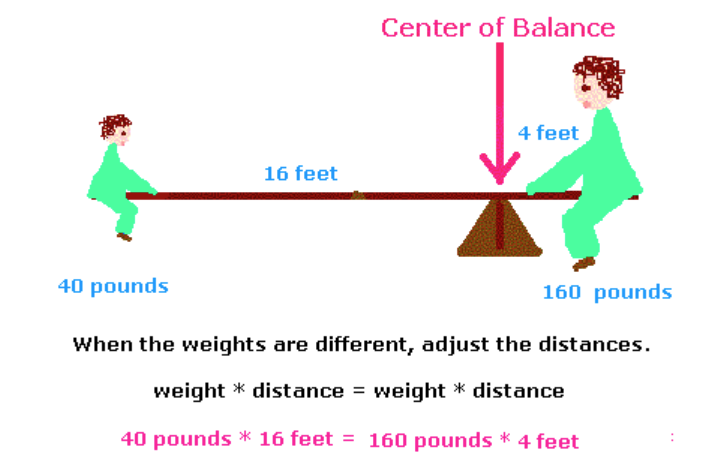
\includegraphics[width=0.8\textwidth]{WD=WD.png}

\section{Ramps}

Ramps, or include planes, let you roll or slide objects up to a higher
level. Steeper ramps give you less mechanical gain. For example, it is much easier 
to roll a ball up a wheel chair ramp than a skateboard ramp.

Assuming the ramp has a constant steepness, the mechanical gain is
equal to the ratio of the length of the ramp divided by the amount
that it rises.

If you assume there is no friction, the force that you push a weight up the ramp will be:

$$F_A = \frac{V}{L} F_G$$

Where $F_A$ is the force you need to push. $L$ is the length of the
ramp, $V$ is the amount of vertical gain, and $F_G$ is the force of
gravity on the mass.

(We haven't talked about the sine function yet, but in case you already know about it: Note that

$$\frac{V}{L} = \sin{\theta}$$

where $\theta$ is the angle between the ramp and level.)

\begin{Exercise}[title={Ramp}, label=ramp]
A barrel of oil weights 136 kilograms. You can push with a force of
up to 300 newtons. You have to get the barrel onto a platform that is 2
meters.  What is the shortest board that you can use as a ramp?
\end{Exercise}
\begin{Answer}[ref=ramp]
  To lift the barrel would require $136 \times 9.8 = 1,332.8$ newtons of force.

  Letting $L$ be the length of the ramp:

  $$300= \frac{2}{L} 1332.8$$

  So $L = 8.885$ meters.
\end{Answer}

\section{Gears}

Gears (which might have a chain connecting them like on a bicycle)
have teeth and come in pairs. You apply torque to one gear, and it
apply torque to another. The torque is increased or decreased based
on the ratio between the teeth on the gears.
% ADD: Driver, Driven, Idler
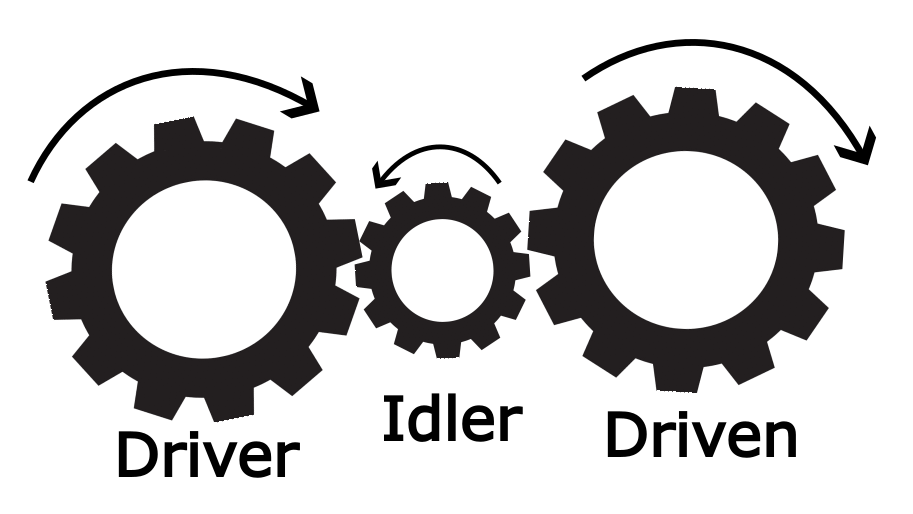
\includegraphics[width=0.8\textwidth]{Gears.png}


If $N_A$ is the number of teeth on the gear you are turning with a
torque of $T_A$, and $N_L$ is the number of teeth on the gear it is
turning, the resulting torque is:

$$T_L = \frac{N_A}{N_L} T_A$$


\begin{Exercise}[title={Gears}, label=gear]

The bicycle is an interesting case because we are not trying to get
mechanical gain. We want to spin the pedals slower with more force.
  
You like to pedal your bike at 70 revolutions per minute. The
chainring that is connected to your pedals has 53 teeth. The
circumference of your tire is 2.2 meters. You wish ride a 583 meters
per minute.

How many teeth should the rear sprocket have?
  
\end{Exercise}
\begin{Answer}[ref=ramp]
  
  $$583 = (70)(2.2)\frac{53}{n}$$
  
Thus $n = 14$ teeth.
\end{Answer}
% KA: https://www.khanacademy.org/science/physics/discoveries/simple-machines-explorations/a/simple-machines-and-how-to-use-this-tutorial

\section{Hydraulics}

In a hydraulic system, like the braking system of a car, you exert
force on a piston filled with fluid. The fluid carries that pressure
into another cyclinder. The pressure of the fluid pushes the piston in
that cyclinder out.
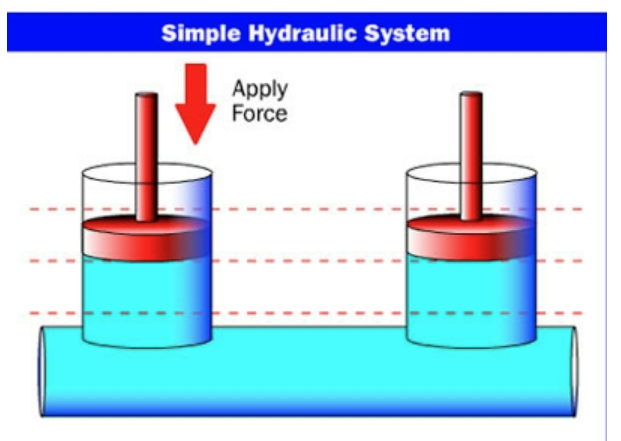
\includegraphics[width=0.8\textwidth]{Hydraulics.png}


The pressure in the hose can be measured in pounds per square inch
(PSI) or newtons per square meter (Pascals or Pa). We will use Pascals.
% ADD: Create a page in the back of the book with units

To figure out how much pressure you create, you divide the force by
the area of the piston head you are pushing.

To figure out how much force that creates on the other end, you
multiply the pressure times the area of the piston head that is
pushing the load.

\begin{Exercise}[title={Hydraulics}, label=hydraulics]

Your car has disc brakes. When you put 2,500,000 pascals of pressure on the
brake fluid, the car stops quickly. As the car designer you would like
that to require 12 newtons of force from the driver's foot.

What should the radius of the master cyclinder (the one the driver is pushing on) be?
\end{Exercise}
\begin{Answer}[ref=hydraulics]
  We are looking for $r$, the radius of the piston head in meters. The area of the piston head is $\pi r^2$.

  The pressure in pascals of the brake fluid is given by $12 / (\pi r^2)$.

  $$2,500,000 = \frac{12}{\pi r^2}$$

  So $r = \sqrt{\frac{12}{\pi \times 2.5 \times 10^6}} = 0.001236077446474$ meters.

\end{Answer}
% KA: https://youtu.be/Pn5YEMwQb4Y

\section{Cognitive bias: the bandwagon effect and groupthink}

\newterm{The bandwagon effect} is our tendency to believe the same
things that the people around us believe. This is how fads spread so
quickly: one person buys in, and then the people they know have a
strong tencdency to buy-in as well.

\newterm{Groupthink} is similar: In order to create harmony with the
people around us, we go along with things we disagree with.

It takes a lot perspective to recognize when those around us are
wrong. And it takes even more courage to disagree with them.

